\documentclass{standalone}
\usepackage{pgf-umlcd}
\begin{document}
    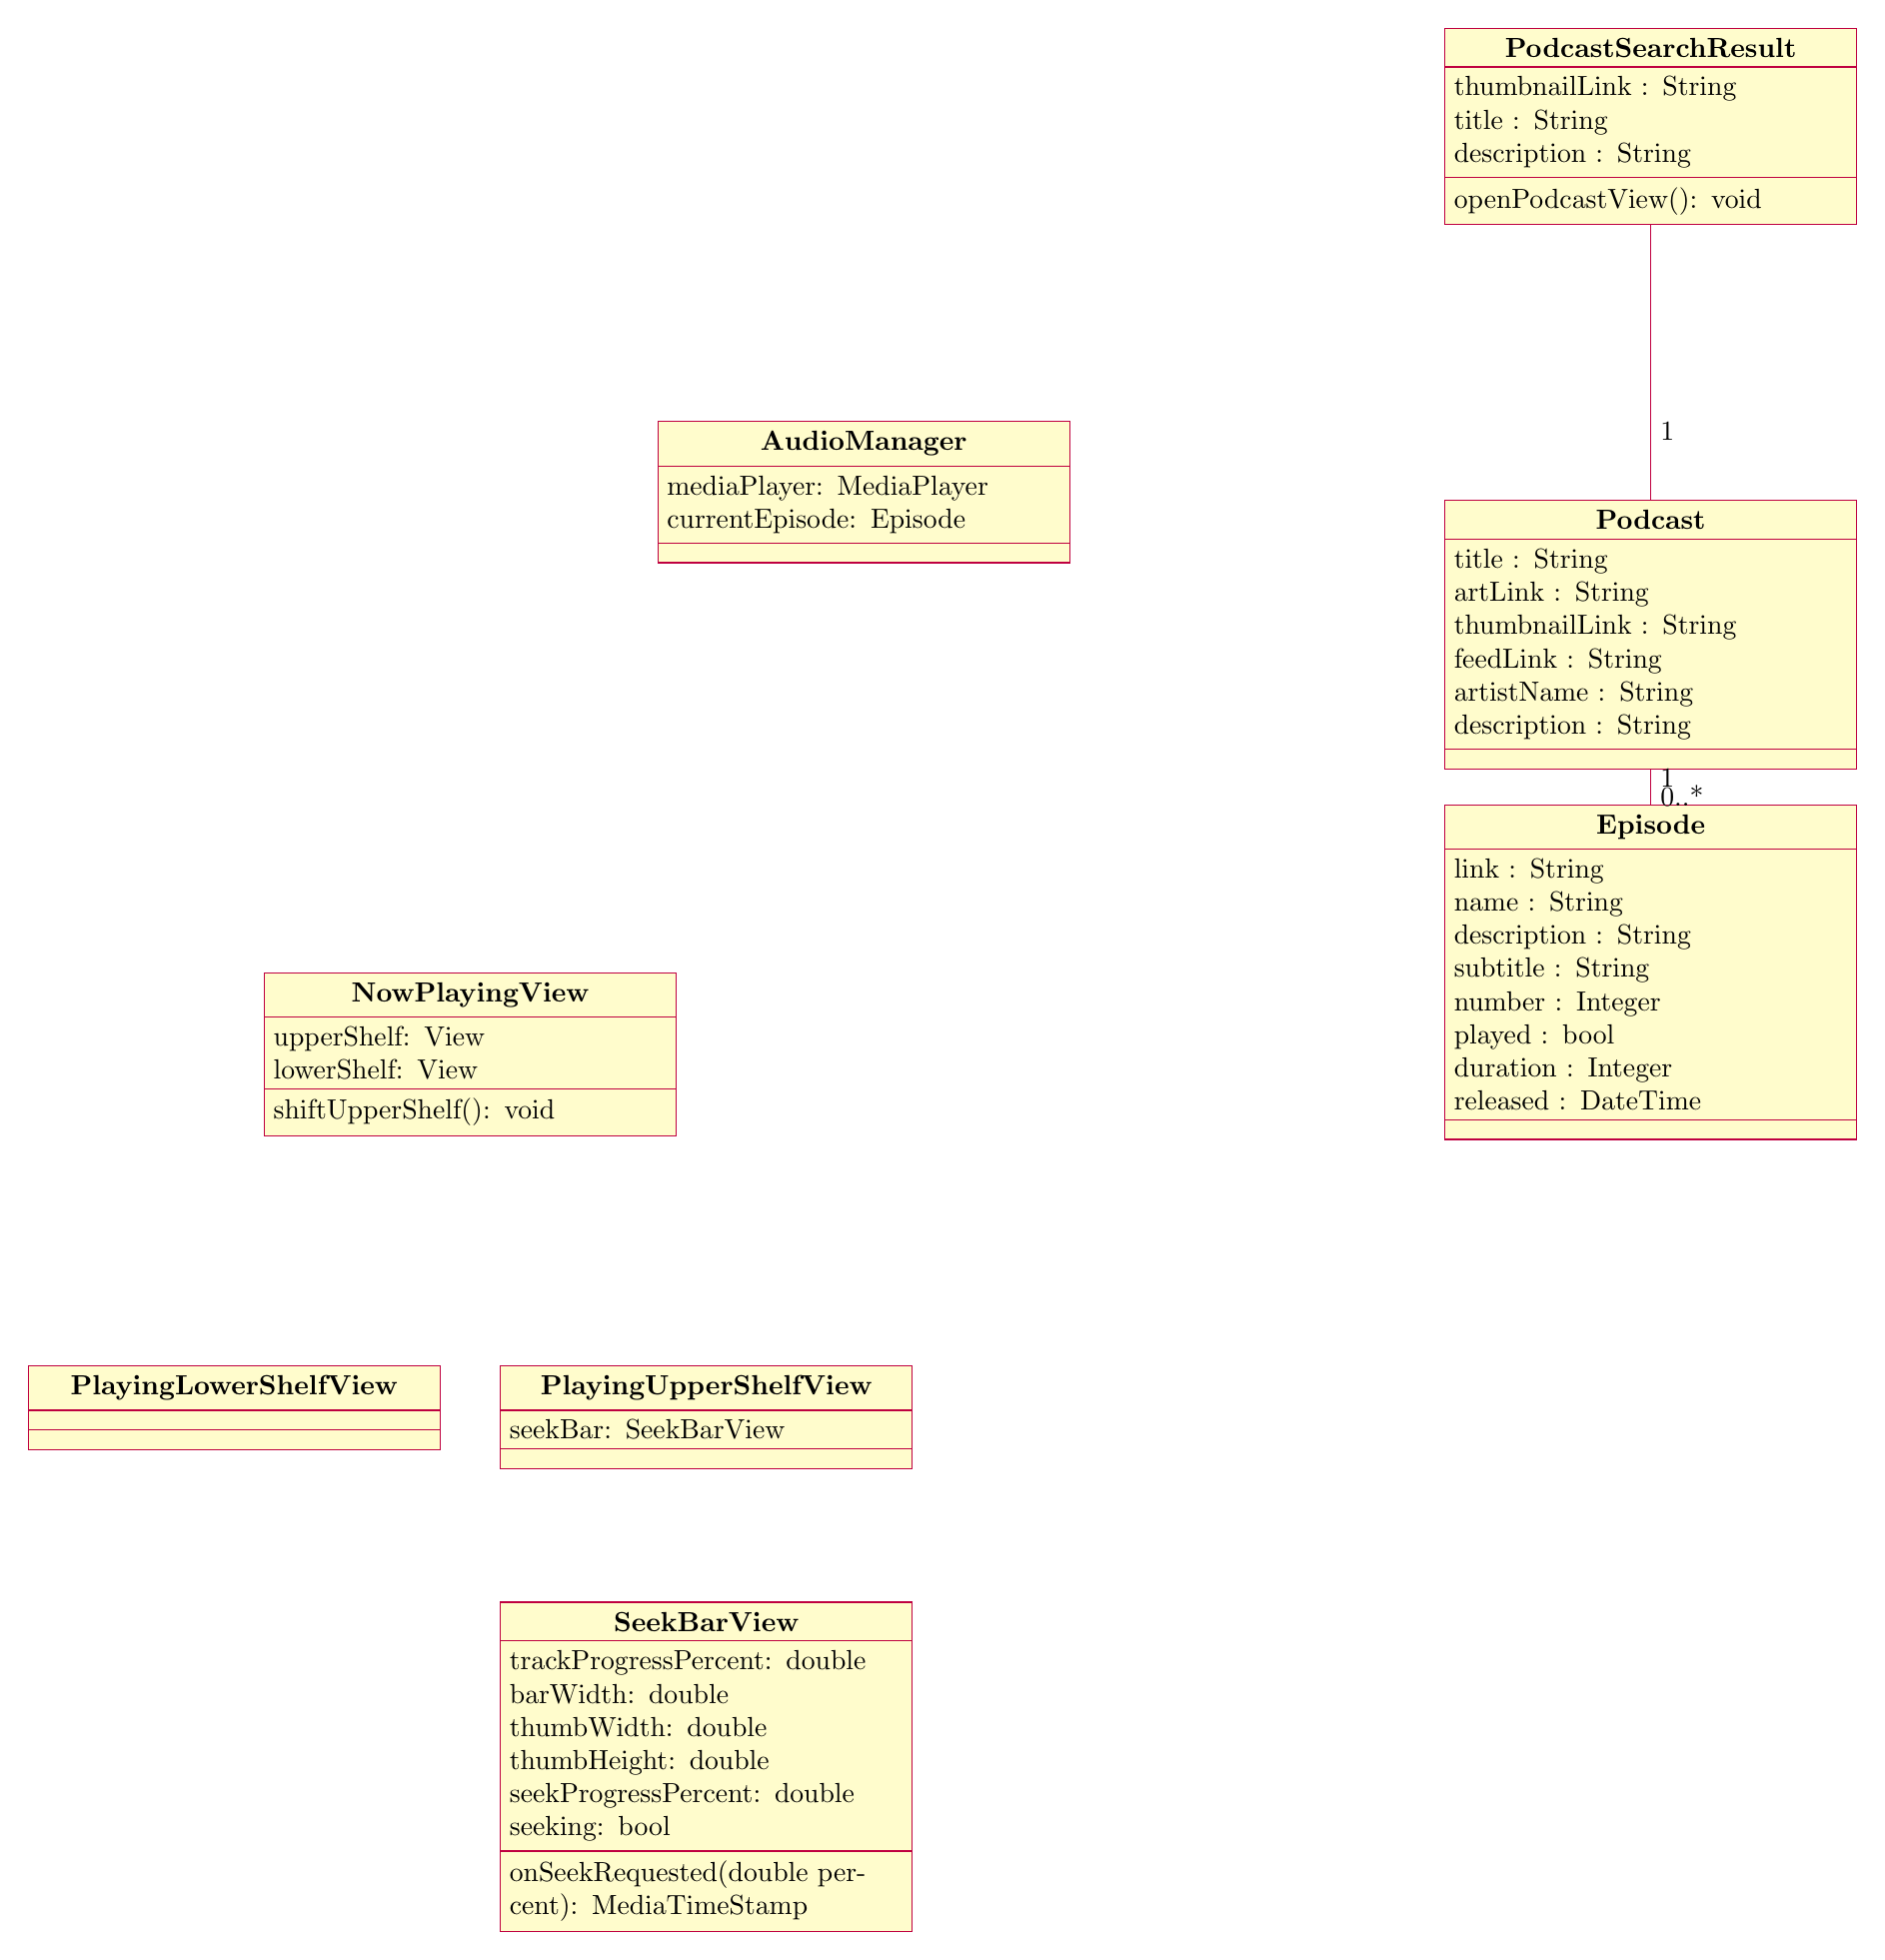
\begin{tikzpicture}[node distance=5cm]
      % AudioManager:
      %   A singleton which controls the playing of podcast audio
      \begin{class}{AudioManager}{-20, 0}
        \attribute{mediaPlayer: MediaPlayer}
        \attribute{currentEpisode: Episode}
        % further methods TBD
      \end{class}
      % NowPlayingView:
      %   Contains the Upper and Lower shelf views
      \begin{class}{NowPlayingView}{-25, -7}
        \attribute{upperShelf: View}
        \attribute{lowerShelf: View}
        \operation{shiftUpperShelf(): void}
        % further methods TBD
      \end{class}
      % PlayingUpperShelfView:
      %   Shows the currently playing podcast's title, description
      %   art, and the SeekBar
      \begin{class}{PlayingUpperShelfView}{-22, -12}
        \attribute{seekBar: SeekBarView}
      \end{class}
      % SeekBarView:
      %   Shows the AudioPlayer's progress through the current file
      %   and allows the user to scrub through the file
      \begin{class}{SeekBarView}{-22, -15}
        \attribute{trackProgressPercent: double}
        \attribute{barWidth: double}
        \attribute{thumbWidth: double}
        \attribute{thumbHeight: double}
        \attribute{seekProgressPercent: double}
        \attribute{seeking: bool}
        \operation{onSeekRequested(double percent): MediaTimeStamp}

      \end{class}
      % PlayingLowerShelfView:
      %   Contains the player controls, meta operations buttons (fav,
      %   share, show chapters), and ChaptersView
      \begin{class}{PlayingLowerShelfView}{-28, -12}
      \end{class}
      % ChaptersView:
      %   Displays all of the chapter related tag/metadata information
      %   on the currently playing audio file
      % PodcastSearchResult:
      %   Represents one result in the list of results displayed when
      %   when searching for a podcast
      \begin{class}[text width=5cm]{PodcastSearchResult}{-10, 5}
        \attribute{thumbnailLink : String}
        \attribute{title : String}
        \attribute{description : String}
        \operation{openPodcastView(): void}
      \end{class}
      
      % Podcast:
      %   describes a whole podcast
      \begin{class}[text width=5cm]{Podcast}{-10, -1}
        \attribute{title : String}
        \attribute{artLink : String}
        \attribute{thumbnailLink : String}
        \attribute{feedLink : String}
        \attribute{artistName : String}
        \attribute{description : String}
      \end{class}
      % Episode:
      %   describes a podcast episode
      \begin{class}[text width=5cm, below of=Podcast]{Episode}{-10, -5}
        \attribute{link : String}
        \attribute{name : String}
        \attribute{description : String}
        \attribute{subtitle : String}
        \attribute{number : Integer}
        \attribute{played : bool}
        \attribute{duration : Integer}
        \attribute{released : DateTime}
      \end{class}
      \association {Podcast}{1}{}{Episode}{0..*}{}
      \association {PodcastSearchResult}{}{}{Podcast}{1}{}
    \end{tikzpicture}
\end{document}





